%%
%% Author: thompson
%% 26.10.17
%%

% Preamble
\documentclass[11pt]{article}

% Packages
\usepackage{a4wide}
\usepackage[utf8]{inputenc}
\usepackage[ngerman]{babel}
\usepackage{scrextend}      % Intending
\usepackage{graphicx}

% Document
\begin{document}

\section{ISO-OSI Referenzmodel}
    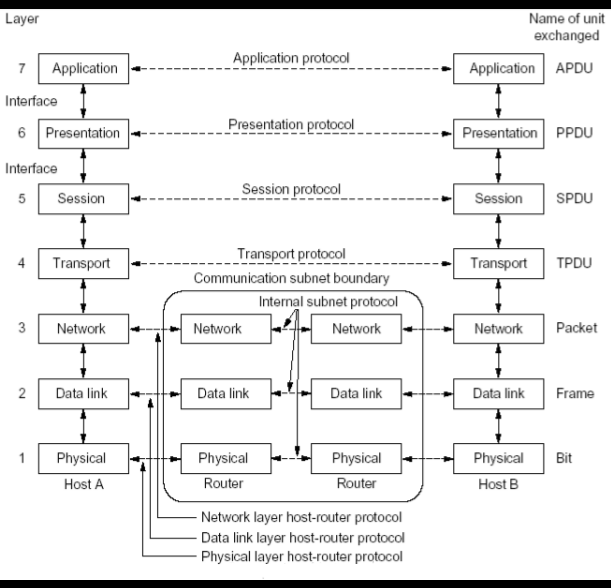
\includegraphics[width=\textwidth]{ISO_OSIReferenceModel.png}

    Das ISO-OSI Referenzmodell besteht aus verschiedenen Anwendungsschichten:
    \begin{enumerate}
        \item \textbf{\underline{Physical Layer}}\\
        Dieser Layer beschreibt die fundamentale Netzwerkkommunikation. Datentransfer via
        physischem Layer sind reine Bitstreams.

        \emph{Hardware}:
        \begin{addmargin}[1em]{1em}
            PHY-Chip: Ein PHY implementiert die Funktionen Senden und Empfangen von Daten zwischen
            Geräten mithilfe des Datalink Layers (MAC, LLC). Es enkodiert und dekodiert einkommende
            Übertragungen und Galvanische Trennung (Blockt ungewollten Datenempfang).
        \end{addmargin}

        \emph{Protokolle}:
        \begin{addmargin}[1em]{1em}
            Integrated Services Digital Network: Internationaler Standard für Datenübertragung \& Telefonie
            Universal Serial Bus: Bussystem von Verbindungen um Daten zu übertragen
            Bluetooth, Ethernet, ...
        \end{addmargin}

        Grundsätzlich wird alles Hardwaretechnische über diese Schicht definiert - Kein Anschluss zum Router,
        eine unterbrochene Kabelverbindung, u.s.w..

        \item \textbf{\underline{Data Link Layer}}\\
        Der Datenlink nutzt Frames zur Übertragung von Datensätzen. Frames bestehen aus einer gewissen Anzahl
        an Bit-Blöcken und einer Prüfsumme, welche die korrekte Datenflussübertragung gewährleistet.
        Fehlerbehafte Frames können anhand dieser Summe erkannt werden und der DLL kann das jeweilige Paket verwerfen
        oder sogar korrigieren.
        Im Falle des Verwerfens ist es allerdings nicht vorgesehen das jeweilige Frame neu anzufordern.

        Mithilfe der 'Data Flow Control' kann man die Dynamik der Frameübertragung steuern, etwa wie schnell
        Blöcke verschickt werden.

        \emph{Hardware}:
        \begin{addmargin}[1em]{1em} % Left & right
            Bridges \& Switches: Arbeiten via Media Access Control(MAC) oder Logical Link Control(LLC).\\
            Die MAC-Bridge schützt gegen Kollisionen via Aufteilung des Netzes in verschiedene Kollisionsdomänen, d.H.
            ein Paket geht nur in das Netz, in welchem sich der tatsächliche Empfänger befindet.\\
            Die LLC-Bridge dient der Koppelung zweier Teilnetze mithilfe verschiedener Zugriffsverfahren, wie
            Token-Passing (Tokens werden zwischen Sendern gewechselt und dementsprechend startet Datenverkehr) oder
            Carrier Sense Multiple Access/Collision Detection (CSMA/CD; Typischer Router mit x-Medien).\\
        \end{addmargin}

        \emph{Protokolle}:
        \begin{addmargin}[1em]{1em}
            HDLC - High-Level Data Link Control: Transmition of sync/async frames\\
            SDLC - Synchronous Data Link Control: Bitsynchron \& Serielle Übertragung\\
            DDCMP - Digital Data Communications Message Protocol: Point-to-Point Transfer (Sicherheit)\\
            SPB - Shortest Path Bridging: Aufbau \& Konfig. + Multipath Routing\\
        \end{addmargin}
        \emph{Normen}: IEEE, FDDI (Fiber Distributed Data Interface), ISO\\

        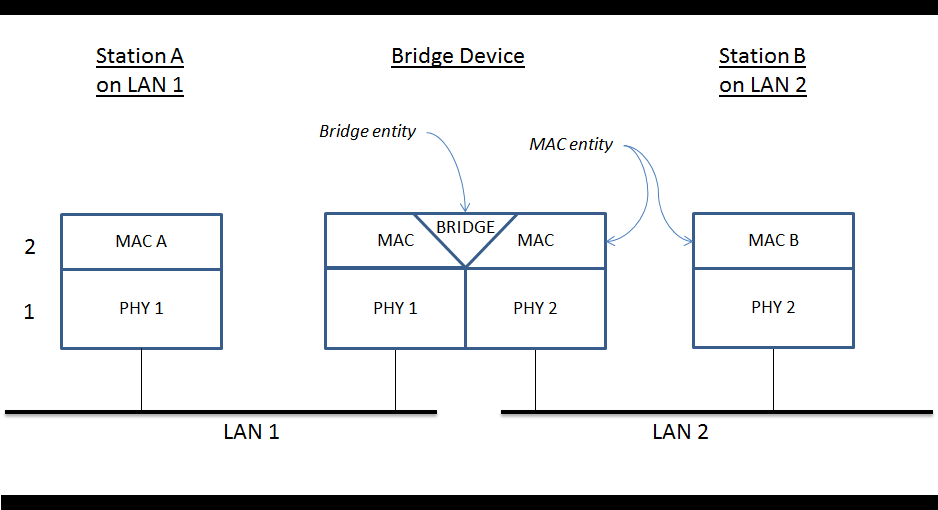
\includegraphics[width=\textwidth]{Network_Bridging.png}
        \footnote[1\small \emph{Schemata of Bridge/Switch inside a Network}]{By Crvincenzi - MS Powerpoint, CC BY-SA 3.0, https://commons.wikimedia.org/w/index.php?curid=25610536}

        \item \textbf{\underline{Network Layer}}\\
        Der Network Layer behandelt die Weiterleitung und Routing durch multiple Zwischenmedien innerhalb
        eines Netzwerkes.

        \emph{Funktionalitäten}:
        \begin{addmargin}[1em]{1em}
            - CL-mode: Verbindungslose Kommunikation, über (TCP-)IP\\
            - Hostadressierung, jeder Host ist einzigartig identifizierbar\\
            - Weiterleitung: Partitionierung von Netzwerken in Subnetzwerke und Weiterleitung
            von Daten über Gateways und Router\\
        \end{addmargin}

        \item \textbf{\underline{Transport Layer}}\\
        Die Transportschicht beschreibt den konkreten Datentransfer von A nach B, genannt "Windowing": Wieviele Daten geschickt oder empfangen werden,
        wann Daten gesendet werden, u.s.w..

        \emph{Protokolle}:
        \begin{addmargin}[1em]{1em}
            - Transmission Control Protocol: TCP/IP - Datentransfer wird kontrolliert weitergegeben. Wird das Paket falsch oder garnicht
            empfangen, so wird eine Anfrage geschickt welche das Datenpaket neu schickt.
            Es gibt Flow- und Congestioncontrol. Grundsätzlich genutzt bei HTTP, FTP, SMTP.\\
            - User Datagram Protocol: UDP/IP - Datentransfer wird losgeschickt, ohne Kontrolle ob das Datenpaket tatsächlich ankommt.
            Es gibt also weder Flow- noch Congestioncontrol.\\
        \end{addmargin}

        \item \textbf{\underline{Session Layer}}\\
        Der Sitzungsschicht beschreibt alles rund um das öffnen, schließen und managen von Sessions zwischen Usern.
        Es handelt sich dabei um einen anhaltenden Dialog der Geräte.

        \emph{Protokolle}:
        \begin{addmargin}[1em]{1em}
            - ISO 8326 - OSI protocol suite: Neuverbindungsaufbau nach Störungen
            - ZIP - Zone Information Protocol (AppleTalk)
        \end{addmargin}

        Wenn man beispielsweise eine Website aufruft, so startet der Layer eine 'Session' mit dem jeweiligen Webserver.

        \item \textbf{\underline{Presentation Layer}}\\
        Die Präsentationsschicht dient der Darstellung der Übertragenen Daten, auch 'Syntax Layer' genannt.
        Durch Konventionen wie ISO, ASCII oder EBCDIC werden die Bitcodes in erste Strukturen umgewandelt.

        Alles was im Rahmen des eigenen Betriebssystemes passiert.

        \item \textbf{\underline{Application Layer}}\\
        Die Applikationsschicht spezifiziert die genutzten Protokolle und Schnittstellen innerhalb der Kommunikation
        zweier Usern, üblicherweise via Internet Protocol Suite: TCP/IP und Open Systems Interconnection Model: OSI

        Prinzipiell alles womit der User direkt arbeitet, z.B. FireFox, Chrome, Skype, Outlook, ...
    \end{enumerate}

    Die 5. und 6. Schicht wird meist impliziert.

\end{document}